\section{Confronto Space Gap con Distanze di Sicurezza}
In questa sezione viene analizzato il comportamento del modello confrontando lo 
Space Gap simulato con quello reale e con le principali definizioni di distanza di sicurezza. 
L'obiettivo è valutare quanto il modello mantenga distanze prudenziali rispetto a riferimenti teorici e pratici.
\\\\
\noindent In Figura \ref{fig:security_distance} sono riportati:
\begin{itemize}
    \item lo \textbf{Space Gap simulato}, estratto da \texttt{dataset\_simulazione} (linea blu);
    \item lo \textbf{Space Gap reale}, estratto da \texttt{dataset\_reale} (linea gialla);
    \item la \textbf{distanza di sicurezza secondo l'ACI} \cite{distanza_di_sicurezza_aci} (linea celeste), calcolata come:
    \[
        d_{sicurezza}[\mathrm{m}] = \left( \frac{v_t(\mathrm{ego}) \, [\frac{\mathrm{km}}{\mathrm{h}}]}{10} \right)^2
    \]
    \item la \textbf{distanza di sicurezza didattica}, insegnata nelle 
    scuole guida \cite{distanza_di_sicurezza_patente} (linea verde), calcolata come:
    \[
        d_{sicurezza}[\mathrm{m}] = \frac{v_t(\mathrm{ego}) \, [\frac{\mathrm{km}}{\mathrm{h}}]}{10} \cdot 3
    \]
\end{itemize}

\noindent La velocità utilizzata per il calcolo delle distanze di sicurezza è la \texttt{ego\_velocity} simulata.

\begin{figure}[H]
    \centering
    \adjustbox{center}{
        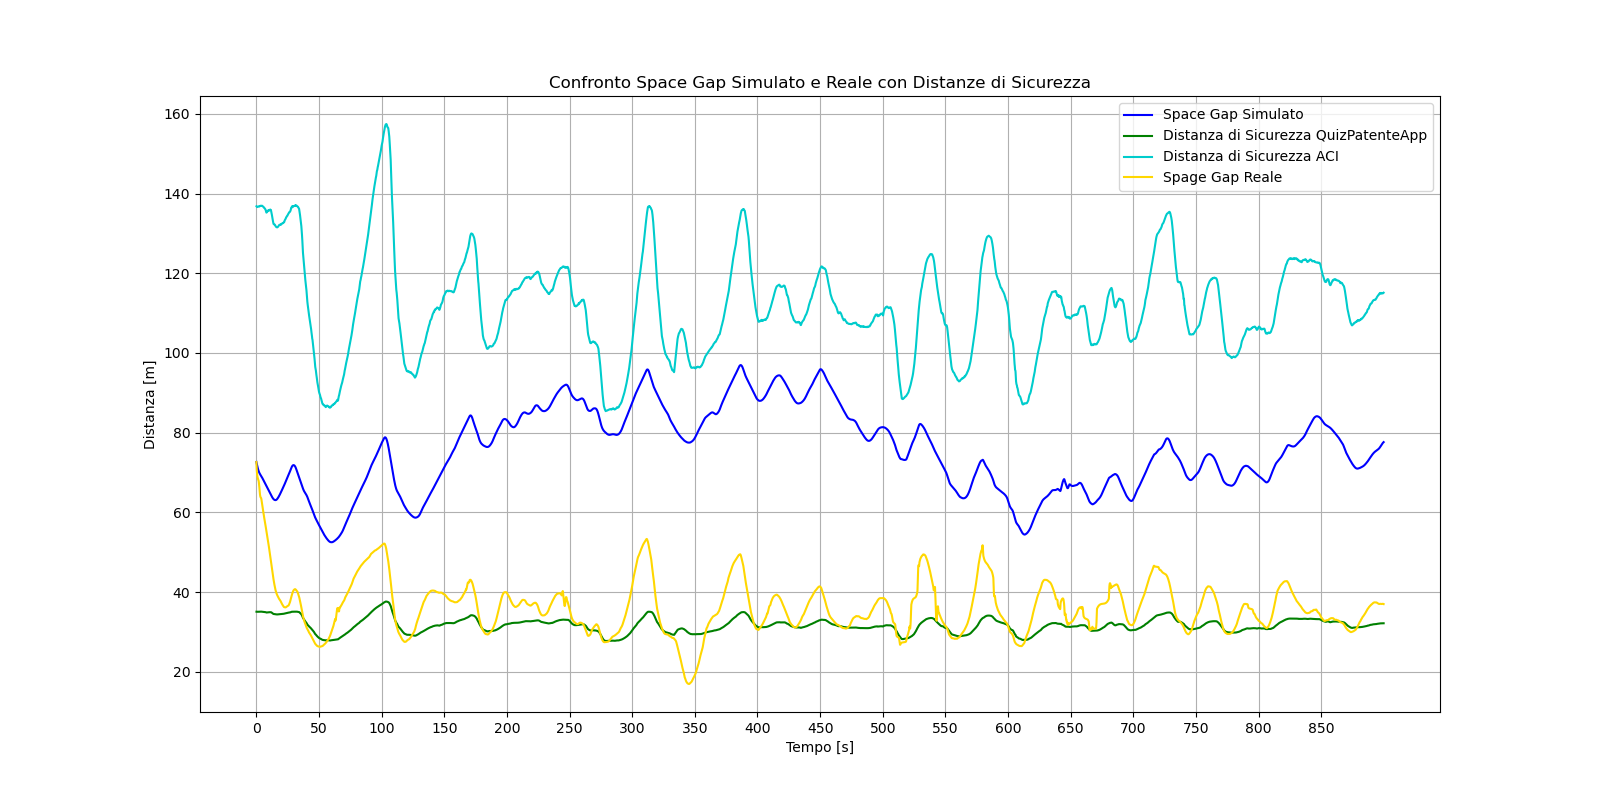
\includegraphics[width=1.25\linewidth]{simulation/leader_comparison/security_distance.png}
    }
    \caption{Confronto Space Gap con le distanze di sicurezza}
    \label{fig:security_distance}
\end{figure}
\noindent Dal grafico emergono alcune osservazioni significative.  
\\\\
\noindent In primo luogo, lo  \textbf{Space Gap simulato} (linea blu) risulta sistematicamente superiore 
allo  \textbf{Space Gap reale} (linea gialla), con una differenza media di circa \(\mu = 39.325 \, \mathrm{m}\) 
e una deviazione standard \(\sigma = 11.519 \, \mathrm{m}\).  
Ciò indica che il modello tende a mantenere una distanza più conservativa rispetto all'ACC reale.
\\\\
\noindent Confrontando lo Space Gap simulato con le due principali definizioni di distanza di sicurezza, si nota che:

\begin{itemize}
    \item rispetto alla formula ACI (linea celeste), la distanza simulata è mediamente 
    inferiore di \(\mu = -35.849 \, \mathrm{m}\) (\(\sigma = 12.194 \, \mathrm{m}\)).  
    Questo significa che, pur essendo superiore allo Space Gap reale, il modello non rispetta le condizioni 
    più restrittive imposte dall'ACI, particolarmente conservative;
    \item rispetto alla regola adottata nei quiz della patente (linea verde), lo Space Gap 
    simulato è mediamente superiore di \(\mu = 43.998 \, \mathrm{m}\) (\(\sigma = 9.960 \, \mathrm{m}\)), 
    evidenziando come il modello si comporti in modo più prudente rispetto alle indicazioni didattiche.
\end{itemize}

\noindent  Nel complesso, il grafico mostra che il modello di simulazione adotta una strategia intermedia: 
più cauta rispetto al comportamento reale osservato, ma meno restrittiva rispetto alle indicazioni ACI.  
Questa caratteristica suggerisce un compromesso tra realismo e sicurezza, coerente con l'obiettivo di simulare 
un sistema ACC (Adaptive Cruise Control) che non sia né troppo aggressivo né eccessivamente conservativo.